\documentclass[xcolor={dvipsnames,table},c,compress,colorlinks]{beamer}
\usepackage{xspace}
\usepackage{comment}
\usepackage{tikz}
\usetikzlibrary{shapes,arrows,positioning}
\usepackage{colortbl}
\graphicspath{{art-images}}

%----------------------------------------------------------------------
% Set up the listings package
\usepackage{listings,bera}
\lstset{ basicstyle=\ttfamily\color{white}% for 'normal' code
       , xleftmargin=0.5em%         left indent, so line number isn't lost
       , xrightmargin=0.5em%        right indent
       , numbers=none%              numbering is not needed on short slides
       , tabsize=2%                 don't waste space with huge tabs
       , stringstyle=\color{yellow}%            for delimeted strings
       , showstringspaces=false%                do not use undercap as space 
       , keywordstyle=\color{green}%            for identified keywords
       , commentstyle=\itshape\color{SkyBlue}%  for comments
       }
\lstloadlanguages{[ISO]C++, bash, Perl}
\lstdefinelanguage{FHiCL}
{
  sensitive = true,
  morekeywords={T, F, true, false, BEGIN_PROLOG, END_PROLOG},
  morecomment=[l]{\#},
  morestring=[b]",
  % moredelim=[s]{\{}{\}},
  % moredelim=[s]{[}{]},
  otherkeywords={:,@local::,\#include}
}
\lstnewenvironment{cpp}{\lstset {language=[ISO]C++}}{}
\lstnewenvironment{fhicllang}{\lstset {language=FHiCL}}{} 
%----------------------------------------------------------------------
% Font selection
\usepackage[T1]{fontenc}
\usepackage{textcomp}
\usepackage{palatino}

%----------------------------------------------------------------------
% Beamer theme control
%----------------------------------------------------------------------
\setbeamercolor*{structure}{fg=OliveGreen!70!black}
\useinnertheme{rounded}
\usecolortheme{dark}
\usefonttheme{structureitalicserif}
\usefonttheme{serif}
%  Turn off the navigation symbols
\setbeamertemplate{navigation symbols}{}
\setbeamertemplate{footline}[frame number]
% Use greyed-out overlays
\setbeamercovered{invisible}

%----------------------------------------------------------------------
% My own macros.
%----------------------------------------------------------------------
%\newcommand{\productname}[1]{\textsc{#1}\xspace}
\newcommand{\productname}[1]{\textbf{\textcolor{cyan}{#1}}\xspace}
\newcommand{\cmd}[1]{\texttt{#1}\xspace}
\newcommand{\expt}[1]{\textbf{\textcolor{Goldenrod}{#1}}\xspace}
\newcommand{\art}{\productname{art}}
\newcommand{\artdaq}{\productname{artdaq}}
\newcommand{\Rprod}{\productname{R}}
\newcommand{\Sprod}{\productname{S}}
\newcommand{\blankline}{\vskip\baselineskip}
\newcommand{\coverpage}[1]{\begin{frame}\begin{center}\vfill\Large #1\end{center}\end{frame}}
\newcommand{\IF}{\expt{Intensity Frontier}}
\newcommand{\Q}[1]{\textcolor{green}{#1}\xspace}
\newcommand{\A}[1]{#1\xspace}
\newcommand{\cppcode}[1]{\lstinline[language=[ISO]C++,escapechar=|]{#1}}
\newcommand{\term}[1]{\texttt{\bfseries\color{green} #1}\xspace}
\newcommand{\eg}{\textit{e.g.}}
\newcommand{\etc}{\textit{etc.}}
\newcommand{\nova}{\expt{NO$\nu$A}}
\newcommand{\argoneut}{\expt{ArgoNeuT}}
\newcommand{\muboone}{\expt{$\mu$BooNE}}
\newcommand{\larsoft}{\expt{LArSoft}}
\newcommand{\mg}{\expt{Muon g-2}}
\newcommand{\mue}{\expt{Mu2e}}
\newcommand{\cms}{\expt{CMS}}
\newcommand{\rootprod}{\productname{ROOT}}
\newcommand{\cling}{\productname{Cling}}
\newcommand{\dzero}{\expt{D\O}}
\newcommand{\mpi}{\productname{MPI}}
\newcommand{\cmake}{\productname{CMake}}
\newcommand{\make}{\productname{GNU Make}}
\newcommand{\python}{\productname{Python}}
\newcommand{\sqlite}{\productname{SQLite}}
\newcommand{\dsf}{\expt{DS50}}
\newcommand{\lbne}{\expt{LBNE}}
\newcommand{\fhicl}{\productname{FHiCL}}
\newcommand{\ruby}{\productname{Ruby}}
\newcommand{\ups}{\productname{UPS}}
\newcommand{\rups}{\productname{Relocatable UPS}}
\newcommand{\srt}{\productname{SoftRelTools}}
\newenvironment{trythis}%
  {\begin{block}{Try this now!}}%
  {\end{block}}

\newenvironment{sourcefile}%
  {\begin{block}{C++ code}}%
  {\end{block}}
%----------------------------------------------------------------------
% Structural elements for the talk.
%
%    TODO: Learn how to control the institution template, so that
%          it doesn't show up too small.
%----------------------------------------------------------------------

\title{Development tools for \art.}
\author[Green]{Chris Green}
\institute[Fermilab]{SCD-ADSS-SSI}
\date[]{\today}

\usepackage{pgf}
\logo{\pgfputat{\pgfxy(1.2,7.)}{\pgfbox[center,base]{\includegraphics[width=2.in]{fermi-logo-white}}}}
%----------------------------------------------------------------------
% Document begins here...
%----------------------------------------------------------------------

\begin{document}
% Title page
\begin{frame}[fragile,plain]
  \color{structure}
  \begin{columns}[onlytextwidth,b]
    \begin{column}{0.7\textwidth}
      \parbox[t][][c]{\textwidth}{\hspace{.5in}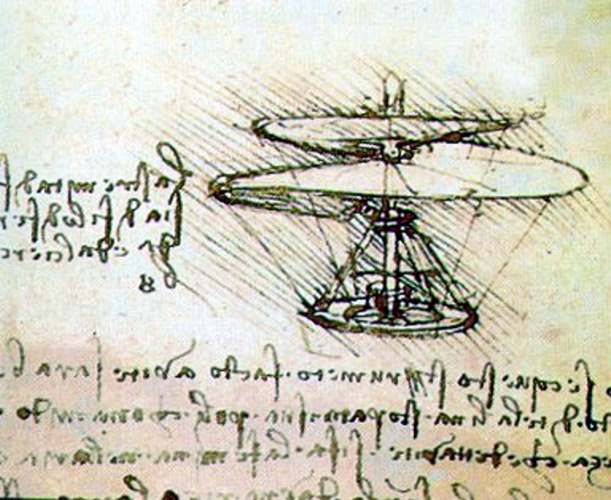
\includegraphics[width=0.4\textwidth]{flyingmachine_l}}
      \\ \vspace{.3in}
      \Huge\textit{Development tools for \art}
    \end{column}
    \begin{column}{0.3\textwidth}
      \hfill
      \mbox{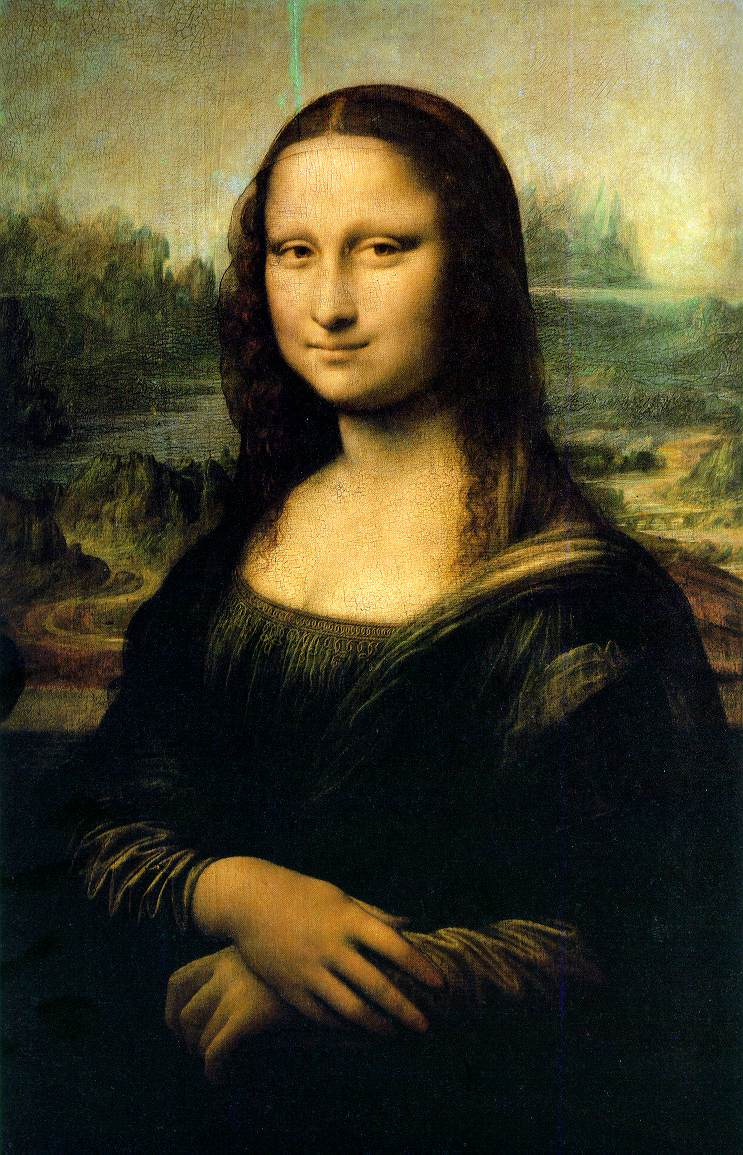
\includegraphics{monalisa_full}}
    \end{column}
  \end{columns}
  \vspace{.3in}
  % \begin{tabular}[b]{lr}
  \begin{columns}[onlytextwidth,b]
    % \parbox[b]{.42\linewidth}{

    \begin{column}{0.45\textwidth}
      Chris Green \\
      SCD-ADSS-SSI
    \end{column}
      % }
    % & %
    \begin{column}{0.55\textwidth}
      \hfill\mbox{\includegraphics[width=2.in]{fermi-credit-white}} \\
    \end{column}
  \end{columns}
  % \end{tabular}
\end{frame}

% Outline
\begin{frame}\frametitle{Outline}
  \begin{itemize}
  \item Motivation.
  \item Details.
  \item Ongoing developments.
  \end{itemize}
\end{frame}

\begin{frame}\frametitle{Why more build tools?}
  \begin{itemize}
  \item Package / install. \\
    \IF experiments want the switchability of UPS but without the \cmd{ups
    declare} commands, and the ability to install multiple packages from tarball.
  \item<2-> Build.
    \begin{itemize}
    \item<3-> Parallel builds.
    \item<4-> Support for testing.
    \item<5-> Build consistency.
    \item<6-> Ease of setup / use.
    \end{itemize}
  \end{itemize}
\end{frame}

\begin{frame}\frametitle{Details: \rups}
  \begin{itemize}
  \item Same \ups, new capabilities.
  \item<2-> No \cmd{prd/}, \cmd{db/} directories
  \item<3-> Each product version has a \cmd{\$\{PROD\_VER\}.version}
    directory instead.
  \item<4-> Use product dependencies (with \cmd{-B} option, \cmd{+}
    qualifiers) to ensure compatible products with error-on-failure.
  \end{itemize}
\end{frame}

\begin{frame}\frametitle{Details: \cmake}
  \begin{itemize}
  \item Built-in support for parallel builds, test.
  \item<2-> Flexible, modular, higher-level than \make.
  \item<3-> Excellent dependency management.
  \item<4-> Install, package, package configuration facilities mesh well
    with \rups.
  \end{itemize}
\end{frame}

\begin{frame}\frametitle{Details: \productname{cetbuildtools}}
  \begin{itemize}
  \item \cmake-based.
  \item<2-> Simple product configuration with \cmd{product\_deps} file,
    listing external package dependencies.
  \item<3-> Straightforward \cmake macros to do most common things: libraries,
    execs, \art plugins, \rootprod dictionaries, tests with pass /
    fail criteria \etc.
  \item<4-> Each package built separately and installed as a \rups product
    to guarantee a consistent build.
    \item<5->Auxiliary scripts for things like version bumps, release
      builds, \etc.
  \end{itemize}
\end{frame}

\begin{frame}\frametitle{Ongoing development}
  \begin{itemize}
  \item Used to build, package and deliver the \art suite to \IF
    experiments.
  \item<2-> Being used on a small-scale by \mg.
  \item<3-> Need a couple more simple macros for common tasks.
  \item<4-> Need a safe scheme for reliable simultaneous multiple
    builds: test releases \textit{a la} \srt are notorious for allowing
    inconsistent builds. May need:
  \item<5-> Library versioning / checking scheme integral to the build
    system.
    \item<6->Sell to \IF experiments.
  \end{itemize}
\end{frame}

\end{document}

%%% Local Variables: 
%%% mode: latex
%%% TeX-master: t
%%% End: 
